\documentclass{beamer}
\usepackage[utf8]{inputenc}
\usepackage[T2A]{fontenc}
\usepackage[english, russian]{babel}
%\usepackage[sfdefault, light]{roboto}
\usepackage{epstopdf}
\usepackage[font={footnotesize}, labelfont={footnotesize}]{caption}
\usepackage[font={footnotesize}, labelfont={footnotesize}]{subcaption}
\usepackage{bm}
\usepackage[absolute,overlay]{textpos}
  \setlength{\TPHorizModule}{1mm}
  \setlength{\TPVertModule}{1mm}

\usepackage{tikz}

% Listings
\usepackage{listings}
\definecolor{codegreen}{rgb}{0,0.6,0}
\definecolor{codegray}{rgb}{0.5,0.5,0.5}
\definecolor{codepurple}{rgb}{0.58,0,0.82}
\definecolor{backcolour}{rgb}{0.95,0.95,0.92}
 
\lstdefinestyle{pythonstyle}{
    backgroundcolor=\color{backcolour},   
    commentstyle=\color{codegreen},
    keywordstyle=\color{magenta},
    numberstyle=\tiny\color{codegray},
    stringstyle=\color{codepurple},
    basicstyle=\scriptsize,
    breakatwhitespace=false,         
    breaklines=true,                 
    captionpos=b,                    
    keepspaces=true,                 
    numbers=left,                    
    numbersep=5pt,                  
    showspaces=false,                
    showstringspaces=false,
    showtabs=false,                  
    tabsize=2
}
\lstset{style=pythonstyle, language=Python}

\graphicspath{ {images/} }
\setbeamertemplate{caption}{\raggedright\insertcaption\par}
\def\figurename{}

\title{Flow networks and the maximum flow problem}
\date[\today]{Практика по дисциплине <<Основы алгоритмов>>\\\today}
\author[Anton]{Першин Антон Юрьевич, Ph.D.}

\institute{Программа <<Большие данные и распределенная цифровая платформа>>\\Санкт-Петербургский государственный университет}

\usetheme{tonythequick}


\begin{document}

\begin{frame}
\titlepage
\end{frame}

\setcounter{framenumber}{0}

\section{}

\begin{frame}{Flow networks}
    \small

    \begin{definition}
        A flow network $G = (V, E)$ is a directed graph in which each edge $(u, v) \in E$ has a nonnegative capacity $c(u, v) \geq 0$. It also has a certain source $s$ and sink $t$.
    \end{definition}

    \begin{itemize}
        \item If $E$ contains an edge $(u, v)$, then there is no $(v, u)$. This is easy to bypass though.
        \item Each vertex lies on some path from $s$ to $t$. As such, a flow network is also connected.
    \end{itemize}

    \begin{figure}[H]
        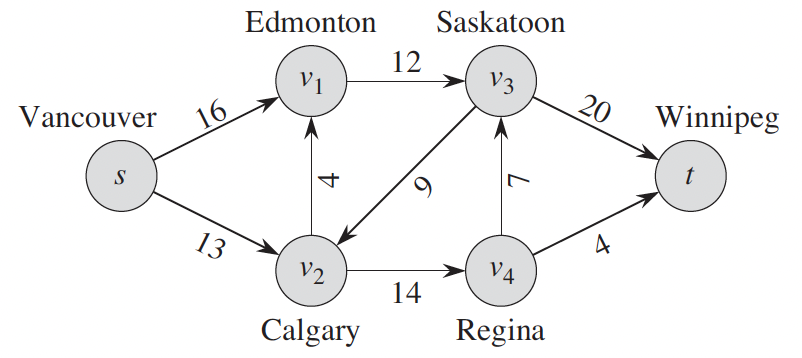
\includegraphics[width=0.7\textwidth]{images/flow_network.png}
    \end{figure}
\end{frame}

\begin{frame}{Flows}
    \small

    \begin{definition}
        A flow in $G$ is a real-valued function $f: V \times V \to \mathbb{R}$ that satisfies the following properties:
        \begin{enumerate}
            \item Capacity constaint: for all $u, v \in V$, we require $0 \leq f(u, v) \leq c(u, v)$.
            \item Flow conservation: for all $u \in V \backslash \{s, t\}$, we require
            \begin{equation}
                \sum_{v \in V} f(v, u) = \sum_{v \in V} f(u, v).
            \end{equation}
        \end{enumerate}
        If $(u, v) \notin E$, there can be no flow from $u$ to $v$, so $f(u, v) = 0$.
    \end{definition}
\end{frame}

\begin{frame}{A value of a flow}
    \small

    \begin{definition}
        A value $|f|$ of a flow $f$ is defined as
        \begin{equation}
            |f| = \sum_{v \in V} f(s, v) - \sum_{v \in V} f(v, s).
        \end{equation}
    \end{definition}

%    \begin{itemize}
%        \item If $E$ contains an edge $(u, v)$, then there is no $(v, u)$. This is easy to bypass though.
%        \item Each vertex lies on some path from $s$ to $t$. As such, a flow network is also connected.
%    \end{itemize}

    \begin{figure}[H]
        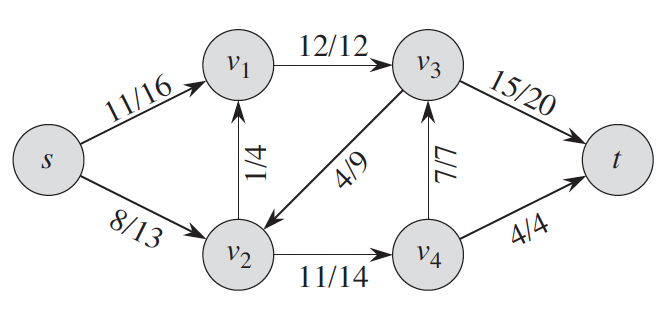
\includegraphics[width=0.7\textwidth]{images/flow.png}
    \end{figure}
\end{frame}

\end{document}
